\section{Benutzertests}

Wie im Dokument ``Ergonomic Criteria for the Evaluation of Human-Computer Interfaces'' spezifiziert, stellt eine kriterienbasierte Bewertungsmethode lediglich einen analytischen Ansatz dar.
Als solche sind die Kriterien nicht dazu gedacht, andere Bewertungsmethoden zu ersetzen.
Daher sind Benutzertests weiterhin notwendig, um die Leistung und Nutzbarkeit einer Schnittstelle zu gewährleisten.
Aus diesem Grund wurden Benutzertests entwickelt, um allgemeine Usability-Probleme zu identifizieren und potenziell Probleme zu erkennen, die nicht von den Kriterien abgedeckt werden.

Das Ziel dieses Tests ist es, die Effektivität, Effizienz und Zufriedenheit mit der Silvanet-Webanwendung mithilfe von echten Nutzern zu quantifizieren.
Zunächst muss jedoch definiert werden, was getestet werden soll und vor allem, wie getestet werden soll.

\subsection{Festlegung der Testabdeckung}

Um relevante und schnelle Tests für die Benutzer durchführen zu können, mussten wir festlegen, auf welche Bereiche der Benutzeroberfläche sich die Tests konzentrieren sollten.
Es erschien uns sinnvoll, eine Gruppenaktivität mit dem Cloud-Team durchzuführen, um Ideen zu sammeln und die am meisten erwähnten auszuwählen.
Um die Brainstorming-Sitzung zu strukturieren und zu vermeiden, dass man sich zu sehr verzettelt, basiert die Aktivität auf der Ideationstechnik namens \textit{Lotus Blossoms}, die es ermöglicht, eine Idee nach der anderen gründlich zu erforschen.
Diese von S. Tatsuno 1990\cite{lotusBlossoms} entwickelte Methode der Ideenfindung lässt sich leicht durch das folgende Flussdiagramm schematisieren.

\begin{figure}[H]
  \centering
  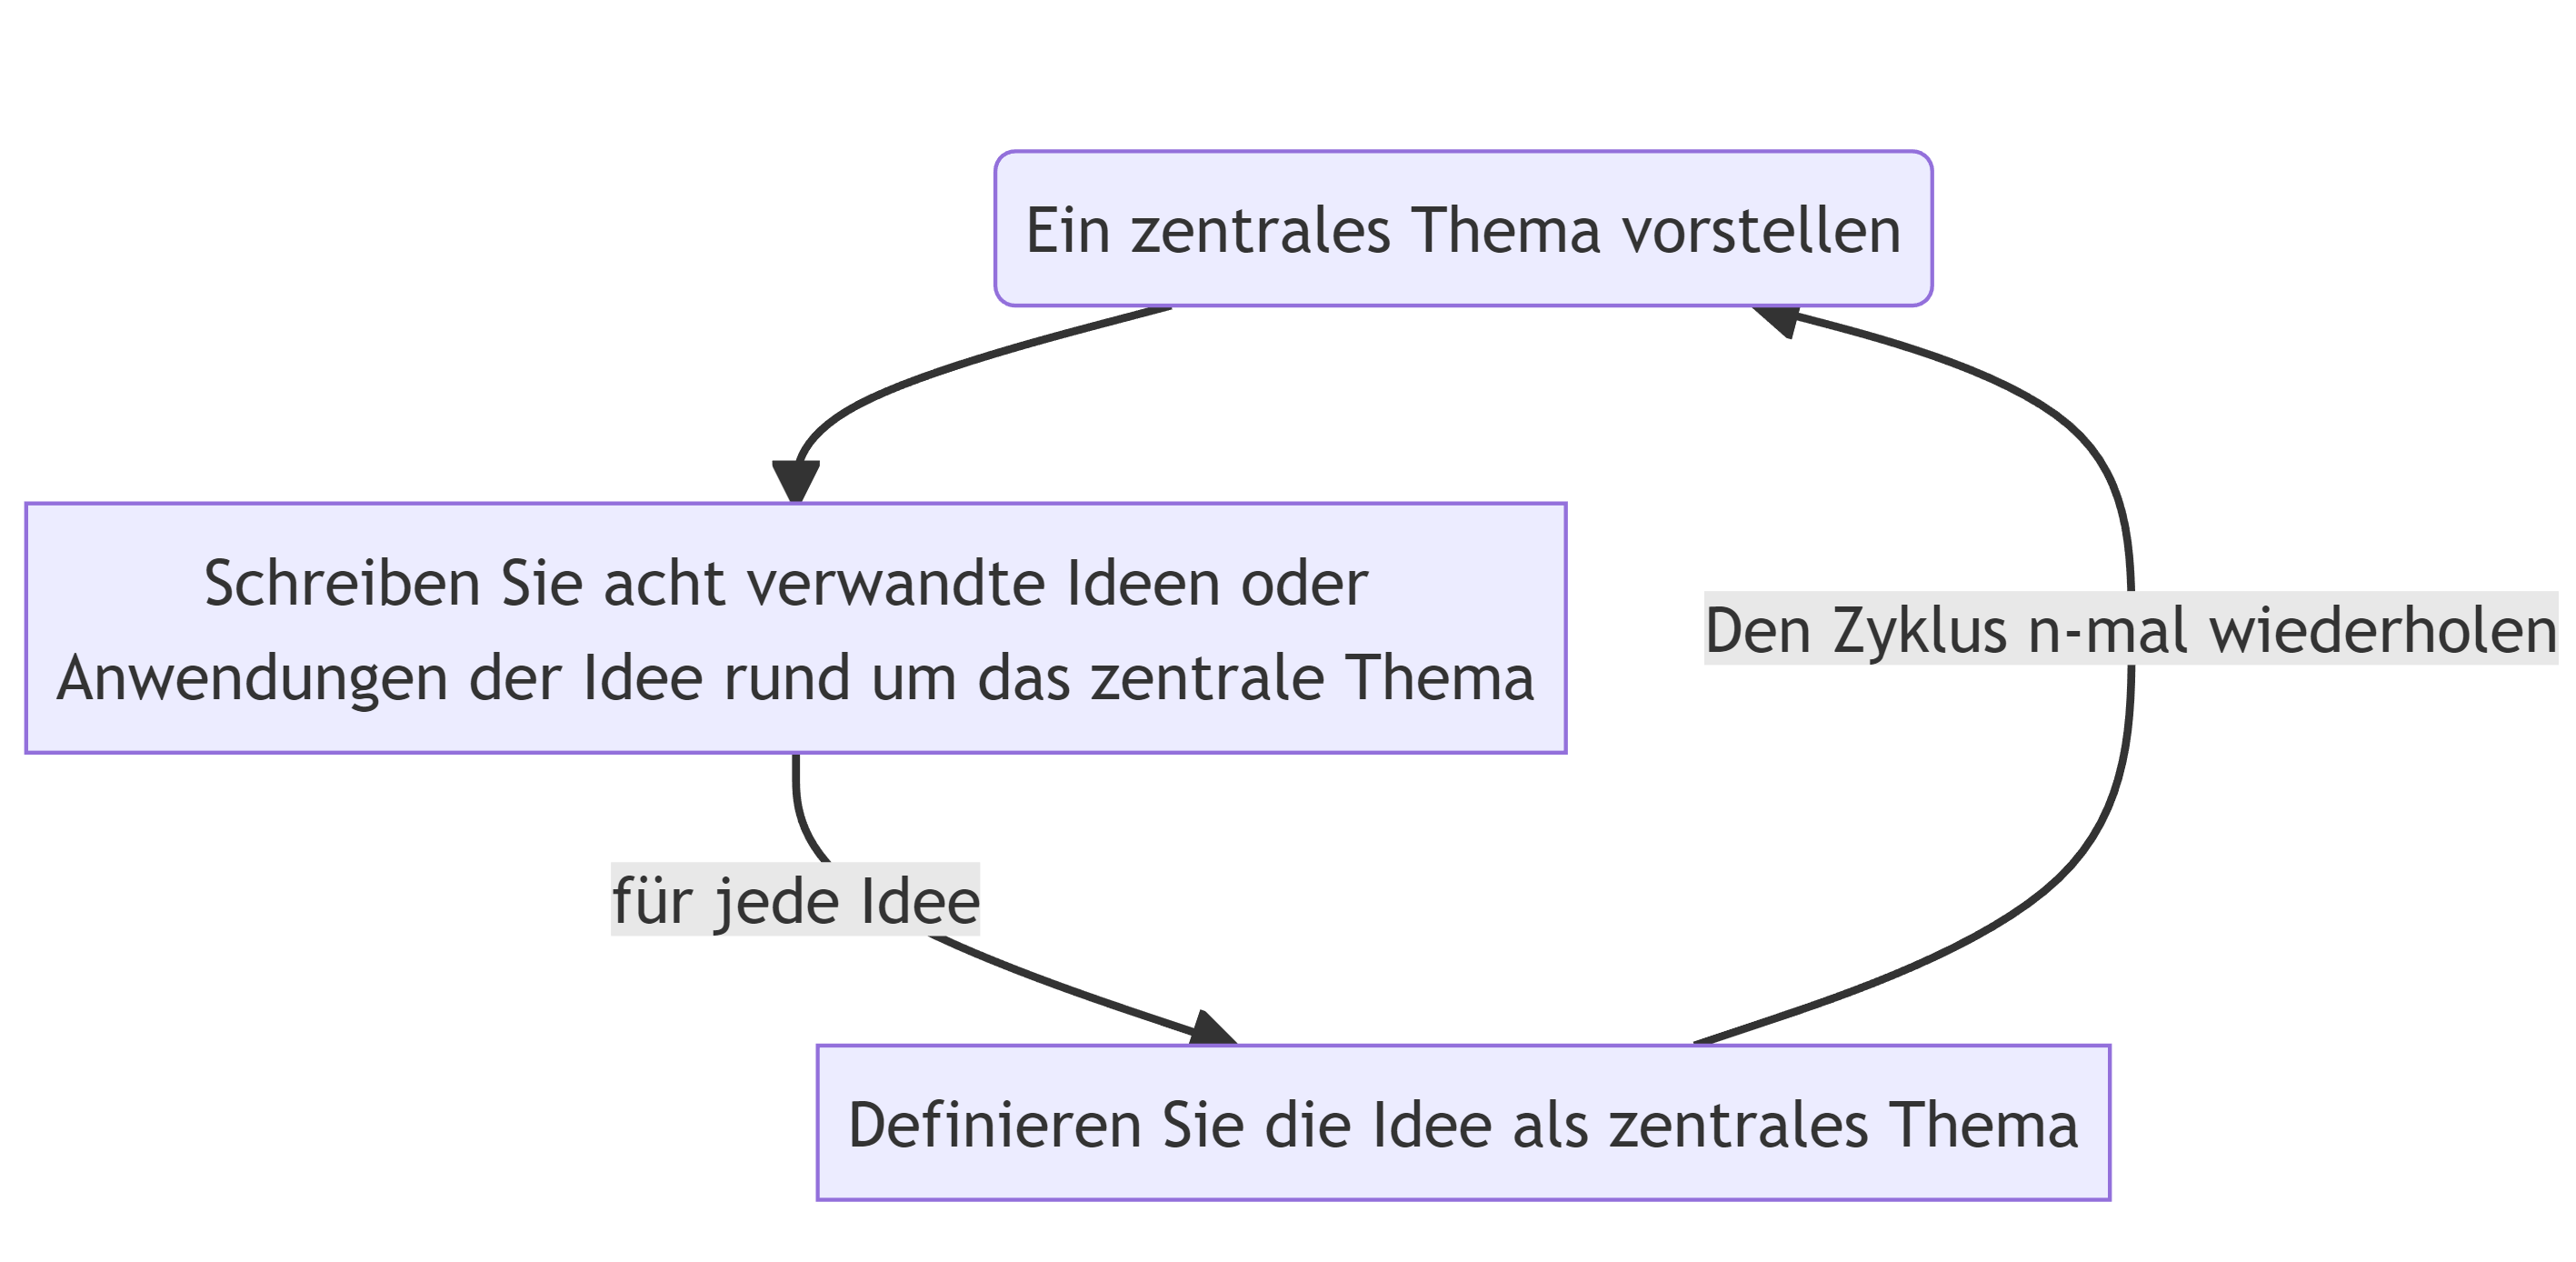
\includegraphics[width=\textwidth]{lotus_blossoms_flowdiagram}
  \caption{Darstellung eines Ideationszyklus mit der Lotus-Blossom-Methode}
  \label{fig:lotus_blossoms_flowdiagram}
\end{figure}

In diesem Fall sollte eine Iteration von zwei Zyklen ausreichen, um die wesentlichen Funktionen der Anwendung zu definieren.
Die erste zentrale Frage wurde im Vorfeld mit der Frage ``Was sind die Ziele des Gesprächs mit dem Kunden über die Anwendung?'' festgelegt.
Aus dieser Frage ergaben sich 6 verschiedene andere Themen:

\begin{itemize}
  \item Welche Informationen über die Geräte sind von Interesse?
  \item Ist die Planung eines \textit{Site} funktionsfähig und die Schnittstelle funktionstüchtig?
  \item Welche kundenorientierten Funktionen sollten den Nutzern zur Verfügung gestellt werden?
  \item Welche Art von Informationen würden Sie im Falle eines Feueralarms interessieren?
  \item Welche Art von Informationen möchten Sie auf dem Dashboard sehen?
  \item Funktioniert die Kartendarstellung gut?
\end{itemize}

\begin{figure}[H]
  \centering
  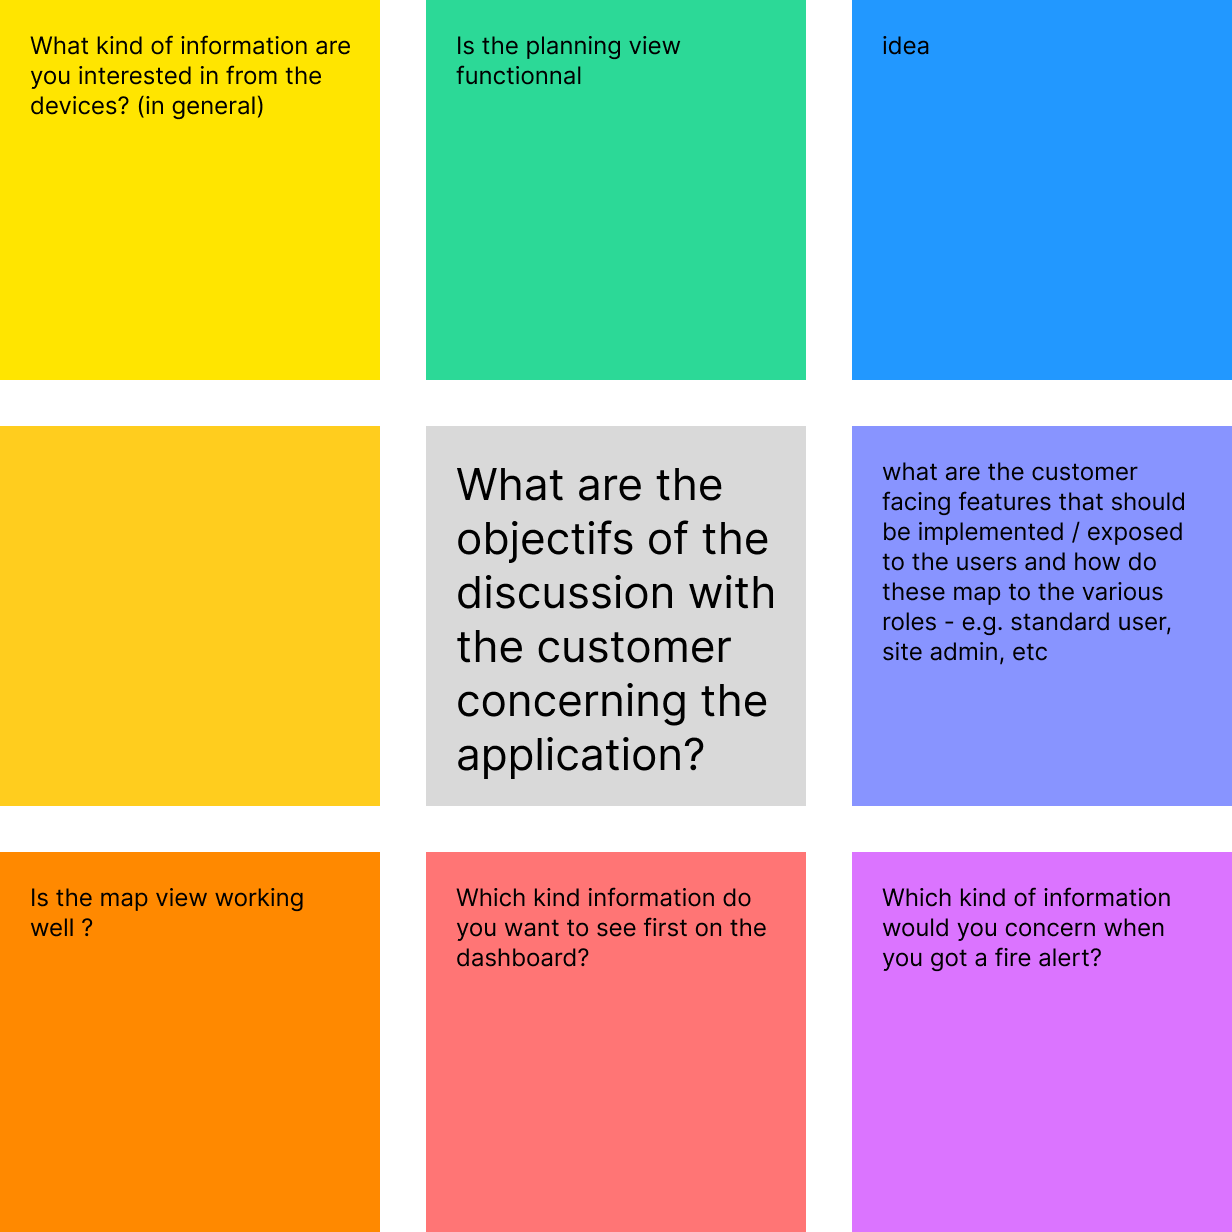
\includegraphics[width=10cm]{dryad_lotus_blossom_cycle_1}
  \caption{Durchführung des ersten Ideationszyklus durch das Cloud-Team von Dryad mit der Lotus-Blossom-Methode}
  \label{fig:dryad_lotus_blossom_cycle_1}
\end{figure}

In der zweiten Iteration wurden mehr Fragen zu den Funktionen der Benutzeroberfläche gestellt, die die genannten Themen beantworten oder näher erläutern können.

\begin{figure}[H]
  \centering
  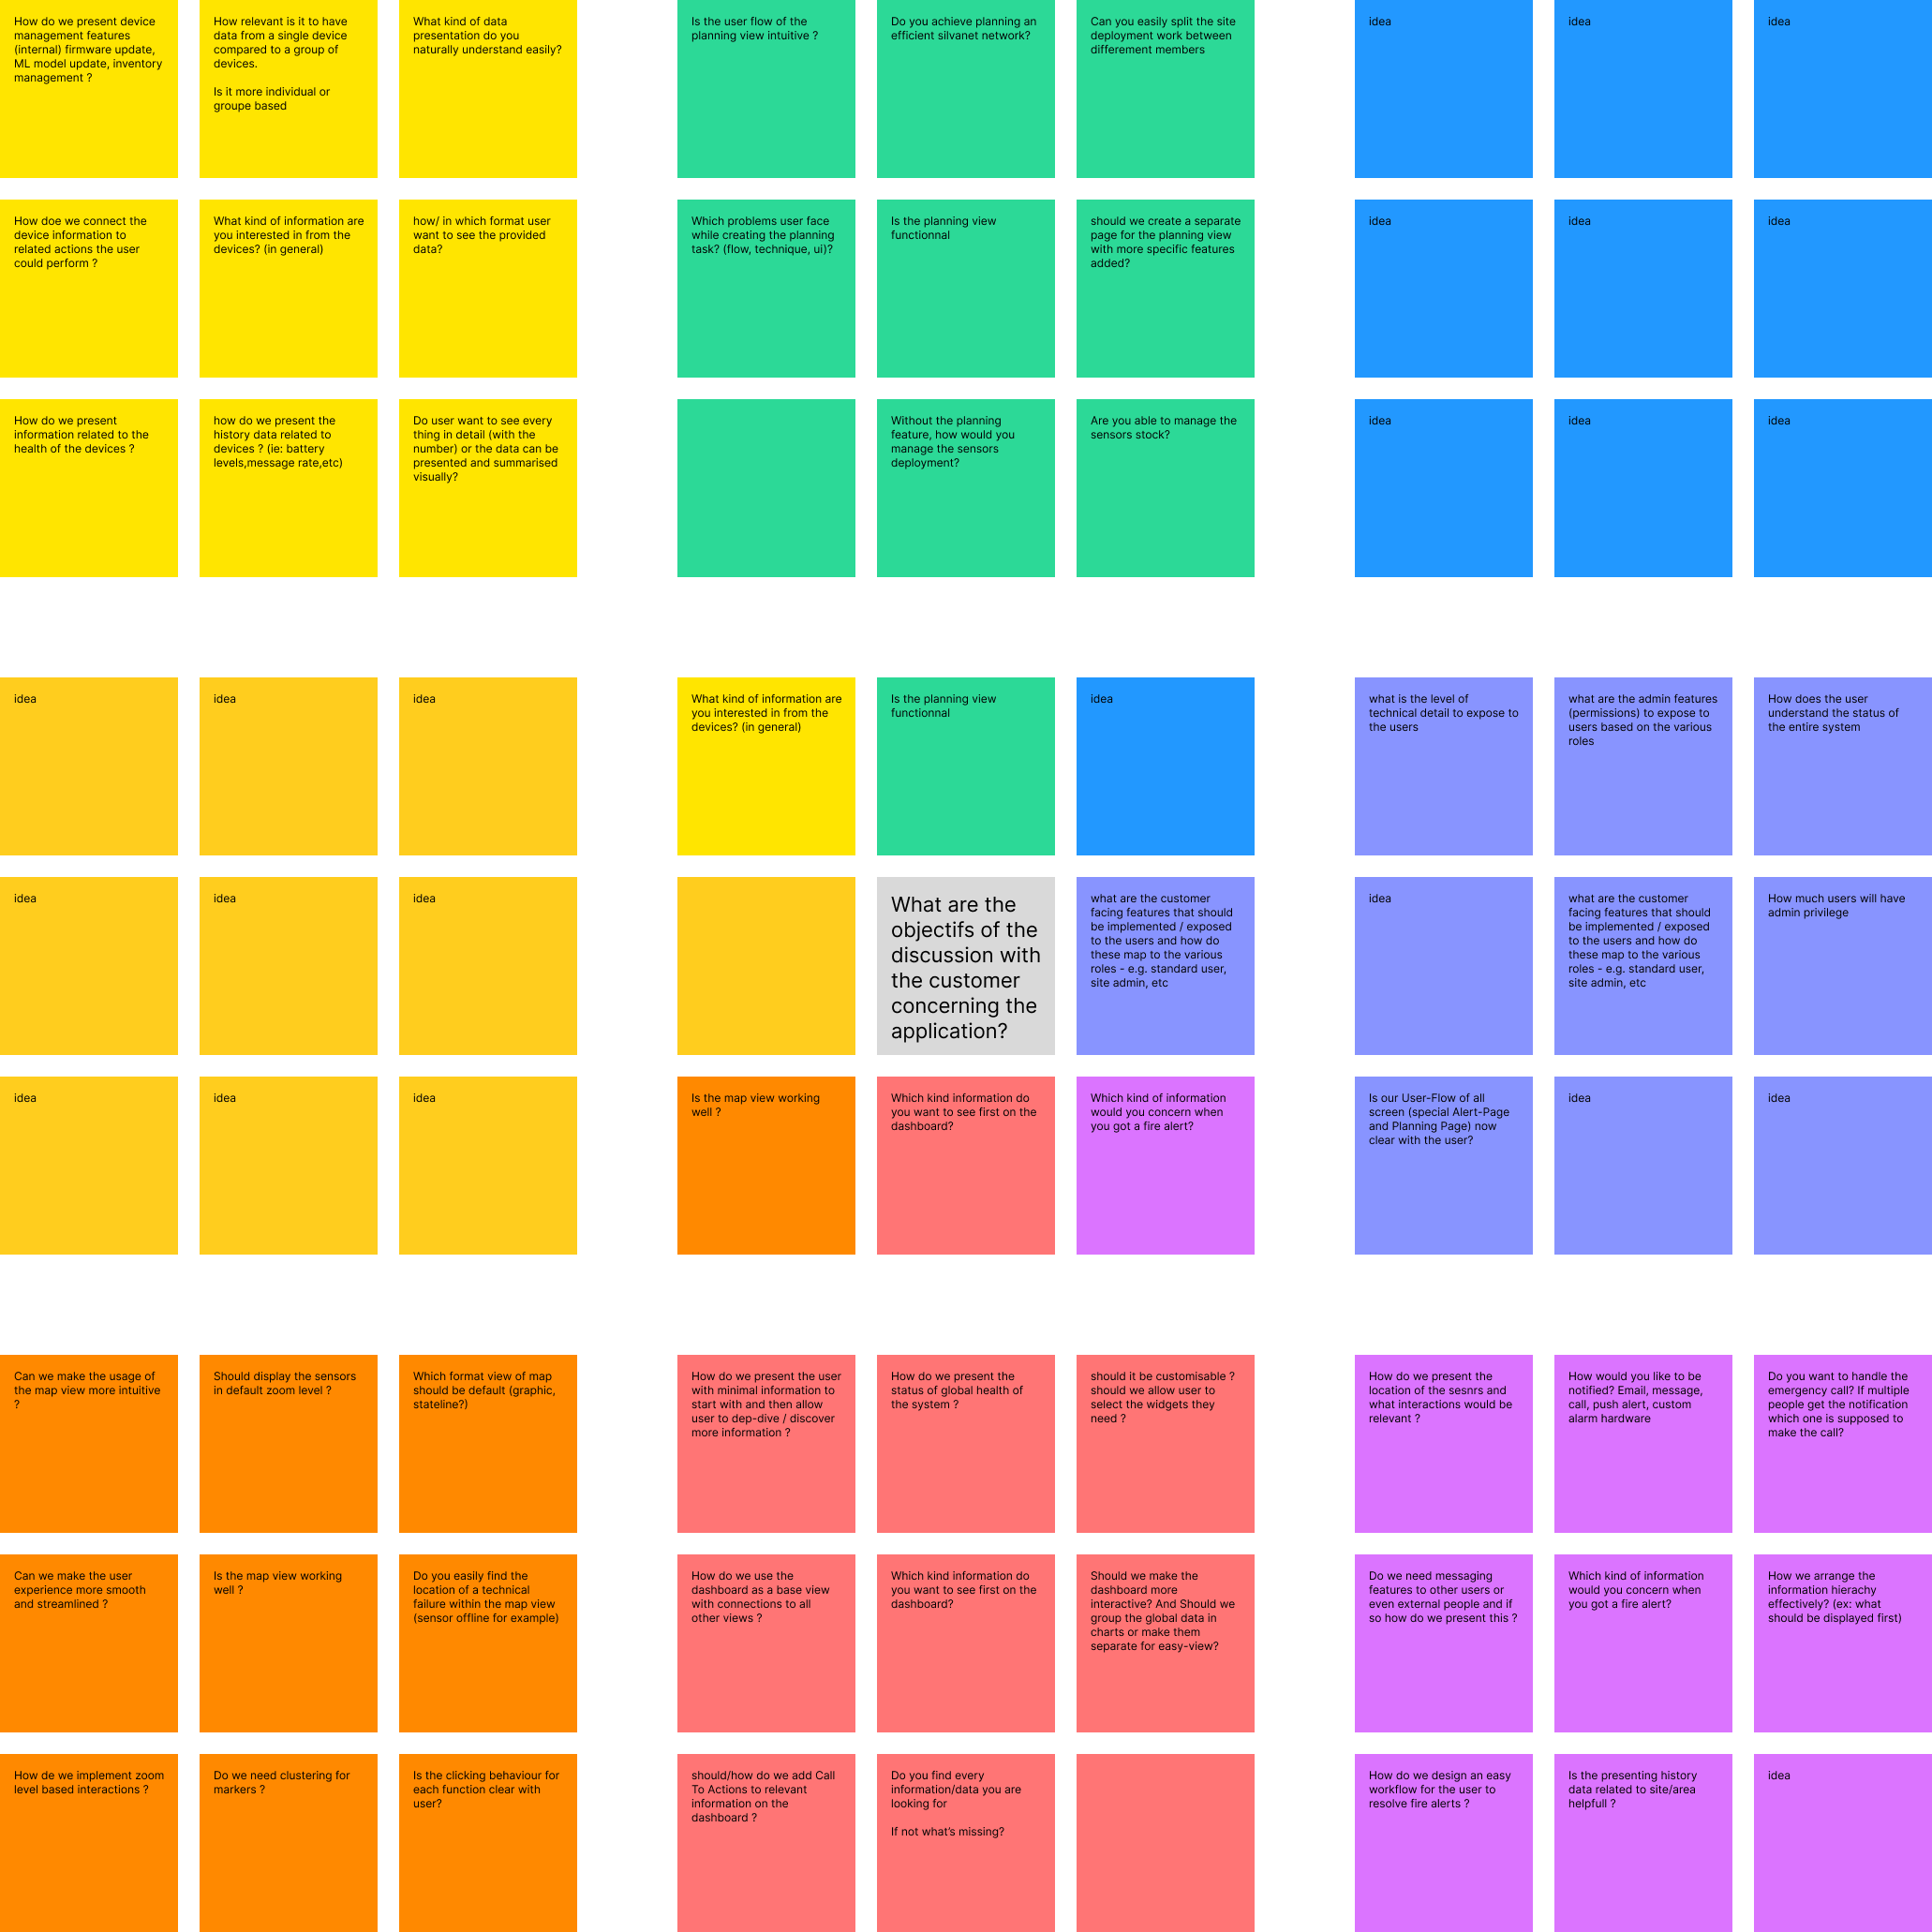
\includegraphics[width=\textwidth]{dryad_lotus_blossom_cycle_2}
  \caption{Durchführung des zweiten Ideationszyklus durch das Cloud-Team von Dryad mit der Lotus-Blossom-Methode}
  \label{fig:dryad_lotus_blossom_cycle_2}
\end{figure}

Die Einzelheiten zu den verschiedenen Blütenblättern der Lotus Blossom des zweiten Zyklus können im Anhang \ref{appendix:lotus_blossom} eingesehen werden.\\

Diese Aktivität ermöglichte es, die Usability-Tests schließlich auf die folgenden Features zu konzentrieren:

\begin{itemize}
  \item \textbf{Planung der Sensoren eines \textit{Site} \ac{UX}}: Die Anwendung bietet dem Nutzer eine Seite, auf der er auf einer interaktiven Karte die neuen Sensoren an einem \textit{Site} so positionieren kann, dass die Erfassungsabdeckung der Sensoren optimiert wird. Dies führt den Nutzer dann durch den Wald zu den Koordinaten, an denen er einen Sensor hoch oben an einem Baum befestigen muss.
  \item \textbf{Relevanz der Information in Alarmsituationen}: Wenn ein Feuer vom System erkannt wird, hat der Benutzer Zugang zu einer Alarmseite, die die Situation mithilfe von Daten und einer interaktiven Karte detailliert darstellt. Es sind auch schnelle Aktionen möglich, wie z.B. die Kontaktaufnahme mit den örtlichen Behörden. Dies betrifft auch Informationen, die per E-Mail an den Nutzer gesendet werden, um ihn über den Alarm zu benachrichtigen.
  \item \textbf{Usability der interaktiven Karte}: Die Anwendung bietet eine Seite, die nur aus einer interaktiven Karte besteht, auf der Sie die verschiedenen \textit{Sites} und Sensoren anhand ihrer geografischen Lage einsehen können.
  \item \textbf{Relevanz von Sensordaten}: In der Anwendung werden die Sensordaten auf unterschiedliche Weise dargestellt. Es wäre interessant, die Strategie zu definieren, die verwendet wird, um diese Daten für den Benutzer relevant zu präsentieren.
\end{itemize}

\subsection{Methoden für Usability-Tests}

Nachdem der Fokus der Usability-Tests festgelegt wurde, ist es nun an der Zeit festzulegen, wie die Tests durchgeführt werden sollen, um in kurzer Zeit möglichst viel relevantes Feedback zu erhalten.
In der von \citeauthor{usability} durchgeführten und in \citetitle{usability} erläuterten Forschung gibt es zwei Techniken, die zusammen eine gute Abdeckung der Usability einer Schnittstelle ermöglichen.

\subsubsection{Qualitative Bewertung}

Die erste besteht in der Entdeckung und Lösung von Usability-Problemen.
Studien zur Problementdeckung zeichnen sich dadurch aus, dass sie sehr informell sind.
Der Schwerpunkt liegt nicht auf der genauen Messung der Leistung oder der Haltung der Teilnehmer, sondern auf einer starken Interaktion zwischen Beobachtern und Teilnehmern.
Die Durchführung dieser Tests ist einfach, da sie auf spezifischen Zielen zur Entdeckung eines Problems basieren, wie z. B. ``Identifizieren Sie einen Sensor an der Schnittstelle, der das Vorhandensein von Rauch detektiert''.
Diese informellen Tests, die mehrmals mit vielen verschiedenen Nutzern wiederholt werden, ermöglichen eine umfassendere Problemerkennung, insbesondere solche, an die die Tester nicht gedacht hätten.
Aus diesem Grund wird eine Reihe solcher Tests für freiwillige Nutzer angeboten.

\subsubsection{Quantitative Bewertung}

Die zweite Methode wird auf einer quantitativen Bewertung der Schnittstelle basieren, die es ermöglicht, eine Usability-Skala zu erhalten, mit der man einfach die Entwicklung der Schnittstelle im Vergleich zur vorherigen Version vergleichen kann, indem man einfach die Bewertungen vergleicht.
Eine weit verbreitete Technik der quantitativen Bewertung basiert auf dem Maß der percuted utilisability, kurz \ac{SUS} genannt\cite{usability}.
\ac{SUS} ist ein standardisierter Fragebogen, der 10 Fünf-Punkte-Items mit abwechselnd positiver und negativer Tonalität enthält. Die Inhalte der Items sind wie folgt:

\begin{enumerate}
  \item I think that I would like to use this system frequently.
  \item I found the system unnecessarily complex.
  \item I thought the system was easy to use.
  \item I think that I would need the support of a technical person to be able to use this system.
  \item I found the various functions in this system were well integrated.
  \item I thought there was too much inconsistency in this system.
  \item I would imagine that most people would learn to use this system very quickly.
  \item I found the system very awkward to use.
  \item I felt very confident using the system.
  \item I needed to learn a lot of things before I could get going with this system.
\end{enumerate}

Für jeden Punkt muss der Nutzer dann eine Bewertung zwischen \textbf{1} und \textbf{5} abgeben, wobei \textbf{1} für \textit{Stimmt überhaupt nicht zu} und \textbf{5} für \textit{Stimme voll und ganz zu} steht. Wenn der Nutzer kein Urteil hat, kann er die Note \textbf{3} geben, die neutral ist.
Wenn Sie fertig sind, können Sie die Gesamtpunktzahl anhand der Punktzahl jedes Items berechnen, die auf eine Skala zwischen 0 und 4 gebracht wird.
Bei positiv formulierten Items (1, 3, 5, 7 und 9) ist der Beitrag zur Punktzahl die Position auf der Skala minus 1.
Bei negativ formulierten Items (2, 4, 6, 8 und 10) ist der Beitrag zur Punktzahl gleich 5 minus der Position auf der Skala.
Um die Gesamtpunktzahl des SUS zu erhalten, muss die Summe der Punktzahlen der einzelnen Items mit 2,5 multipliziert werden.
So reichen die SUS-Scores von 0 bis 100 in Schritten von 2,5 Punkten.\\

Schließlich kann die Punktzahl einer Schnittstelle mithilfe der folgenden Skala adjektiviert werden:

\begin{itemize}
  \item (score <= 25): Unvorstellbar schlecht
  \item (25 < score <= 51,7): Schlecht
  \item (51,7 < score <= 71,7): Fair
  \item (71,7 < score <= 80,7): Gut
  \item (80,7 < score <= 84,1): Ausgezeichnet
  \item (84,1 < score): Das Beste, was man sich vorstellen kann
\end{itemize}

\begin{figure}[H]
  \centering
  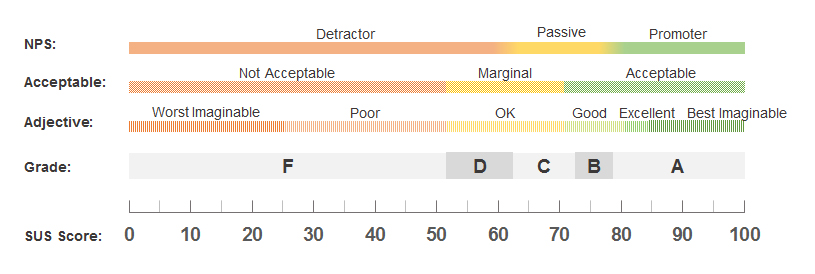
\includegraphics[width=\textwidth]{sus_scala}
  \caption{Noten, Adjektive, Akzeptanz und NPS-Kategorien in Verbindung mit den SUS-Rohwerten\cite{sus_scala}}
  \label{fig:sus_scala}
\end{figure}

\subsubsection{Bewertung durch Vergleich}

Wenn ein Nutzerproblem gut bekannt ist und bereits eine oder mehrere Verbesserungsideen vorgeschlagen wurden, ist es sinnvoll, die relevanteste mithilfe eines Vergleichstests zu bewerten.
Die Idee dahinter ist sehr einfach: Dem Benutzer wird eine Aktion gegeben, die er auf zwei Schnittstellen ausführen muss. Am Ende des Tests wählt der Benutzer aus, welche Schnittstelle er bevorzugt hat.
Wenn die Schnittstellen nicht entwickelt werden, reichen einfache Screenshots zum Vergleich aus.
Dieses Vergleichsverfahren hat einen Namen, der häufiger verwendet wird: \textit{A/B-Testing}.
